%\documentclass[draft]{beamer}
\documentclass{beamer}
  
\usepackage{thumbpdf}           % Thumbnails for PDF versions
\usepackage{hyperref}
\usepackage{pgf}
\usepackage{tikz}
\usepackage{bm}
\usepackage{movie15}
\usepackage{textcomp}

\definecolor{green::dark}{rgb}{0.,0.7,0}

\title{Advanced Amateur Radio Licence}
\author{Rupert Brooks}

%%%%%%%%%%%%%%%%%%%%%%%%%%%%%%%%%%%%%%%%%%%%%%%%%%%%%%%%%%%%%%%%%%%%%%%%%%%%%%%%%%
%\setbeamertemplate{navigation symbols}{}
%\setbeamertemplate{frametitle}[default][right]
\setbeamertemplate{frametitle}{
\begin{flushright}
\insertframetitle\\
{\small \insertframesubtitle}
\end{flushright}
}

\setbeamertemplate{footline}[frame number]

\usefonttheme{professionalfonts}

%\setbeamertemplate{background}
%{
%\put(-10,0){
%\includegraphics[height=0.2\paperwidth]{logo.jpg}
%}%
%\put(0,2){
%\includegraphics[width=0.5in]{MICCAI_Logo_CMYK.pdf}
%}


%%%%%%%%%%%%%%%%%%%%%%%%%%%%%%%%%%%%%%%%%%%%%%%%%%%%%%%%%%%%%%%%%%%%%%%%%%%%%%%%%%
\def\lemma{{\large  \usebeamercolor[fg]{titlelike} Lemma\\}}
\def\proof{{\large  \usebeamercolor[fg]{titlelike}  Proof\\}}
\def\endproof{\qed}

\def\point#1{{\large  \usebeamercolor[fg]{titlelike}  #1\\}}
\def\herepoint#1{{\large  \usebeamercolor[fg]{titlelike}  #1}}

\def\emph#1{{\usebeamercolor[fg]{titlelike}  #1}}

%%%%%%%%%%%%%%%%%%%%%%%%%%%%%%%%%%%%%%%%%%%%%%%%%%%%%%%%%%%%%%%%%%%%%%%%%%%%%%%%%%
\begin{document}

%%%%%%%%%%%%%%%%%%%%%%%%%%%%%%%%%%%%%%%%%%%%%%%%%%%%%%%%%%%%%%%%%%%%%%%%%%%%%%%%%%
\begin{frame}
\maketitle
\end{frame}


%%%%%%%%%%%%%%%%%%%%%%%%%%%%%%%%%%%%%%%%%%%%%%%%%%%%%%%%%%%%%%%%%%%%%%%%%%%%%%%%%%
%% \section*{Outline}
%% \begin{frame}[allowframebreaks]
%% \frametitle{Outline}
%% \tableofcontents
%% \end{frame}
%%%%%%%%%%%%%%%%%%%%%%%%%%%%%%%%%%%%%%%%%%%%%%%%%%%%%%%%%%%%%%%%%%%%%%%%%%%%%%%%%%

\section*{Outline}

\begin{frame}{Outline}{}
\tableofcontents
\end{frame}
%%%%%%%%%%%%%%%%%%%%%%%%%%%%%%%%%%%%%%%%%%%%%%%%%%%%%%%%%%%%%%%%%%%%%%%%%%%%%%%%%%
\section{Components and circuits}

\subsection{Active Components}
\begin{frame}{Tubes}{}
\begin{itemize}
\item Diode: Electrons will flow in a vacuum from a hot cathode to an anode, but not the other way.
\item Triode: Adding a grid in between at a variable voltage, allows to control a large current with
a small current.
\item Tetrodes and pentodes: Operation of the triode has some linearity and other problems. Tetrodes and pentodes add other grids (screens) to clean this up (roughly speaking).
\item The Cathode may be heated separately by the filament, or heater.
\item All this metal junk may have stray capacitance, and require {\em neutralization} in RF work.
\end{itemize}
\end{frame}

\begin{frame}{Grounded Grid amplifier}{}
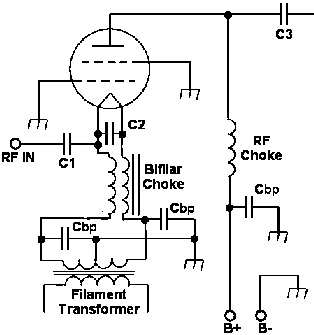
\includegraphics[width=0.6\textwidth]{images/gg1.jpg}
Image taken from \url{http://wb0nni.dakotamade.com/ggbasic.html}.  See there for discussion, also the answer to the grounded grid questions
\end{frame}

\begin{frame}{Semiconductors}{}
\begin{itemize}
\item Semiconductors are materials such as silicon, germanium or gallium arsenide (GHz freq).
\item Note that pure Si is an insulator.  
\item When doped, there are either extra electrons (N-type), or missing electrons (holes) (P-Type)
\end{itemize}
\end{frame}

\begin{frame}{Diodes}{}
\begin{itemize}
\item Hot-Carrier or Schottky - Low forward voltage drop and fast switching.  Cats-whisker detector is a form of Schottky diode.  Good for VHF/UHF mixers and detectors. Metal contact on a single type of doped semiconductor.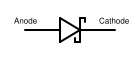
\includegraphics[width=0.15\textwidth]{images/Schottky_diode.png}

\item PIN diode - Have a layer of intrinsic semiconductor between the P and N layers.  Low capacitance and fast switching. Good for RF switch
\item Point-contact diode: Group III metal makes a sharp contact on N-type semiconductor.  Some metal dissolves into the semiconductor generating a small P region.  The 1N34 Germanium diode is an example, makes good RF detectors.
\end{itemize}
\end{frame}

\begin{frame}{Diodes}{}
\begin{itemize}
\item Varactor diode - varies internal capacitance with applied voltage 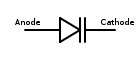
\includegraphics[width=0.15\textwidth]{images/Varactor.png}

\item Zener diode - regulates voltage through breakdown at a specific voltage level via the Zener mechanism, and some avalanche mechanism.
\item Avalanche diode - (not on exam).  Can suppress voltage spikes through avalanche breakdown - not as regulated as Zener.
\end{itemize}
\end{frame}

\begin{frame}{Bipolar Junction Transistor}{}
\begin{itemize}
\item PNP or NPN types. Current positive to negative against the arrow.
\item Allows small base-emitter current to control large collector emitter current.
\item $I_e=I_b+I_c$
\item Common base current gain $\alpha=I_c/I_e$
\item Common emitter current gain $\beta=I_c/I_b=H_{fe}$
\item Common collector current gain $\gamma=I_e/I_b$
\item $\alpha=\frac{\beta}{1+\beta}=\frac{\gamma-1}{\gamma}$
\item $\beta=\frac{\alpha}{1-\alpha}=\gamma-1$
\item $\gamma=1+\beta=\frac{1}{1-\alpha}$
\end{itemize}
\end{frame}

\begin{frame}{Other active components}{}
\begin{itemize}
\item FETs (Field Effect Transistors): A three terminal device, with source, drain and gate.
\begin{itemize}
\item Enhancement mode FET: No channel, no current flows at zero voltage.  Voltage must be applied to create the channel and allow current to flow.
\item Depletion mode FET: Channel, current flows with zero voltage applied.  Voltage must be applied to shut it off (or encourage it)
\item Junction FET: has a PN junction to separate the gate
\item MOSFET: Metal-oxide-semiconductor separates the gate.  Static sensitive.
\end{itemize}
\item SCR: A three terminal (anode, cathode and gate), four layer (PNPN) device.  Once triggered by gate current, behaves like a junction diode.  In amateur radio, frequently used in crowbar overvoltage protection.
\end{itemize}
\end{frame}

\subsection{Transistor Circuit configurations}
\begin{frame}{Common Emitter}{}
\begin{center}
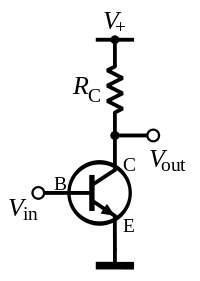
\includegraphics[width=0.25\textwidth]{images/common_emitter.png} \\
{\tiny \url{http://en.wikipedia.org/wiki/File:NPN_common_emitter.svg}}
\end{center}
\begin{itemize}
\item Current amplification $>> 1$. Voltage amplification $>> 1$
\item phase reversal (180 degrees)
\item similar to FET common source
\item in the FET common source, the input impedance is essentially determined by the gate biasing network
\item in the FET common source, output impedance is essentially determined by the drain resistor.
\end{itemize}
\end{frame}

\begin{frame}{Common Base}{}
\begin{center}
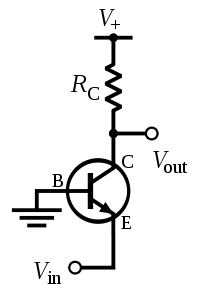
\includegraphics[width=0.25\textwidth]{images/common_base.png}\\
{\tiny \url{http://en.wikipedia.org/wiki/File:NPN_common_base.svg}}
\end{center}
\begin{itemize}
\item Current amplification $< 1$ Voltage amplification $>> 1$
\item no phase shift
\item low input impedance
\item similar to FET common gate
\end{itemize}
\end{frame}

\begin{frame}{Common collector}{}
\begin{center}
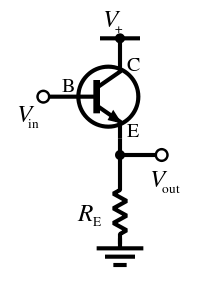
\includegraphics[width=0.3\textwidth]{images/common_collector.png}\\
{\tiny \url{http://en.wikipedia.org/wiki/File:NPN_emitter_follower.svg}}
\end{center}
\begin{itemize}
\item Current amplification $>>1$. Voltage amplification $< 1$
\item no phase shift
\item aka emitter follower
\item similar to FET common drain (source follower)
\end{itemize}
\end{frame}

\begin{frame}{Darlington pair}{}
\begin{center}

\includegraphics[width=0.3\textwidth]{images/Darlington_pair.png}\\
{\tiny \url{http://en.wikipedia.org/wiki/File:Darlington_pair_diagram.svg}}
\end{center}
\begin{itemize}
\item Current amplification $>>1$. Voltage amplification $>> 1$
\item high gain
\item high input impedance
\item low output impedance
\end{itemize}
\end{frame}

\subsection{Amplifier Characteristics}
\begin{frame}{Amplifier classes}{}

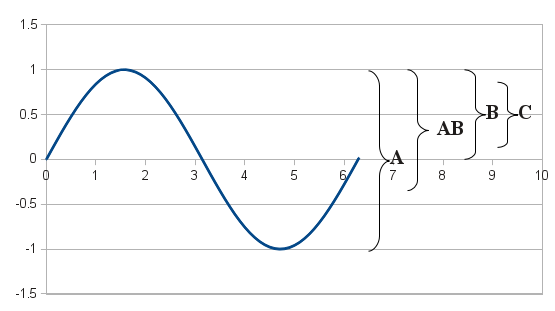
\includegraphics[width=0.6\textwidth]{images/amplifierclasses.png}
\begin{itemize}
\item A: full 360 of phase, most linear, least efficient
\item AB: More than 180 of phase, but less than 360 (SSB)
\item B: 180 of phase
\item C: Less than 180 of phase. Most distortion, most efficient (CW, RTTY or FM)
\end{itemize}
\end{frame}

\subsection{Filters}
\begin{frame}{Filters}{}

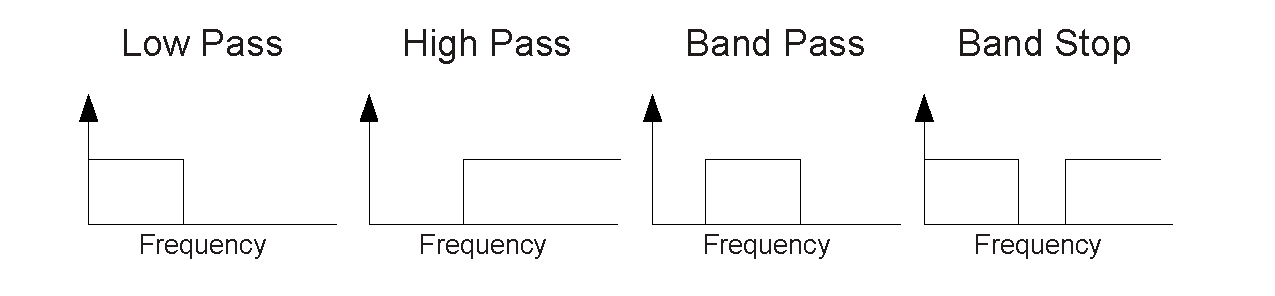
\includegraphics[width=0.8\textwidth]{images/filters.pdf}
\begin{itemize}
\item Butterworth is flat (smooth as butter), but sacrifices steepness of skirts
\item Chebyshev type I is described in the hamstudy notes (passband ripple).
\item Chebyshev type II exists, has stopband ripple instead
\item Both Chebyshevs accept some ripple in return for steep skirts
\item Elliptic filters are a family of filters that range between Butterworth, and the two Chebyshevs at the extremes.
\item Cavity filters and helical resonators are physical objects.  Cavity filters have very narrow BW.
\end{itemize}
\end{frame}


\subsection{Continued}
\begin{frame}{See the hamstudy notes}{}

\begin{itemize}
\item Operational Amplifiers
\item Mixer and frequency multiplier (explain image frequency)
\item Digital Logic
\item Quartz Crystals
\end{itemize}
\end{frame}


%%%%%%%%%%%%%%%%%%%%%%%%%%%%%%%%%%%%%%%%%%%%%%%%%%%%%%%%%%%%%%%%%%%%%%%%%%%%%%%%%%

\section{Meters and Measurement}

\begin{frame}{Voltages and PEP}{}
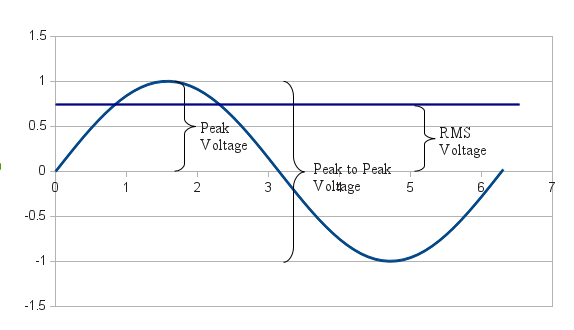
\includegraphics[width=0.8\textwidth]{images/peak2peak.png}
\begin{itemize}
\item Peak Envelope Power: $PEP=E_{RMS}^2/R$
\end{itemize}

\end{frame}

\begin{frame}{See Notes}{}
\begin{itemize}
\item For the rest of the meters, see the hamstudy notes
\end{itemize}

\end{frame}

%%%%%%%%%%%%%%%%%%%%%%%%%%%%%%%%%%%%%%%%%%%%%%%%%%%%%%%%%%%%%%%%%%%%%%%%%%%%%%%%%%

%\section{Modulation}

%\subsection{Rectifiers}
%\begin{frame}{Rectifiers}{}
%\end{frame}

%%%%%%%%%%%%%%%%%%%%%%%%%%%%%%%%%%%%%%%%%%%%%%%%%%%%%%%%%%%%%%%%%%%%%%%%%%%%%%%%%%
\end{document}
 
